\subsection{Equal current dimension: opportunity and access}
The previous preconditioning tests solve the same complete normal equation. We next test the current approximation itself. All selectors use a common full forward residual, total-field material injection, physical material coordinates, and regularization; only the tangent-current Galerkin space changes. The budget $k=4,8,12,16,24,32$ is the actual number of independent complex current columns shared across six illuminations. The quality measure is the gap in the unchanged full quadratic, as defined in the preceding design section.

Sixteen prescribed objects cover smooth Gaussian lobes, touching or separated ellipsoids, shell/layered structures, and asymmetric multiple objects. Each family has two Gaussian and two voxel material tangents. The inverse and data grids are $12^3$ and $14^3$; receivers provide two transverse channels at 64 positions. The latter grid is a finer DDA reference. Initial, pre-fourth-update, and final valid linearizations come from one common full-reference trajectory per object. One reference failed and two state evaluations ended in native process failures. The observed noiseless subset therefore contains 43 of 48 states, 258 of 288 state--budget units, and 15 objects; 13 objects have all three states. Deferred noise checks and these gaps retain their original status.

Receiver singular vectors, a projected receiver/internal proxy, Fourier directions, current-energy POD, and ten random seeds supply current-based controls. Transfer-magnitude, lifted joint-spectrum, first-order gain, and finite-gain rules share the declared candidates. The finite rules estimate full-quadratic gain using an independent 64-column current reference, with zero or limited complete-model probes. Each addition is rescored with full Schur coupling. A generic primal--dual current POD/Galerkin adaptation uses the same information and total dimension. Separately charged offline search evaluates actual current Galerkin spaces in a declared dictionary union, including tested baseline spaces; it is best-found rather than globally certified.

For each object we sum paired absolute gaps and divide by the corresponding receiver sums, then report the median of object ratios. The receiver rule was locked using development data. Intervals use 10,000 object-cluster bootstrap replicates; states and budgets are repeated observations within each object. The offline search achieves ratio 0.4242, with 95\% interval $[0.2832,0.5710]$. Both finite-gain variants have ratio 1.0947 and win on six of 15 objects. The no-probe interval is $[0.3814,1.8308]$; the limited-probe interval is $[0.3814,1.8601]$. Their median captured fraction of resolvable same-domain oracle improvement is $-0.1396$, retained without clipping. Searching with complete information demonstrates opportunity; the tested reduced-reference rule does not reliably recover it.

\begin{table}[tbp]\centering\caption{Observed noiseless object-median full-quadratic gap ratios relative to development-locked receiver selection at the same actual current dimension. Smaller is better. The search is offline; both finite rules are separately evaluated.}\label{tab:current-budget}
\footnotesize\setlength{\tabcolsep}{3pt}\begin{tabular}{rrrrr}\toprule
$k$ & \shortstack{Finite\\no probes} & \shortstack{Limited\\probes} & \shortstack{Offline\\search} & \shortstack{Primal--dual\\POD}\\\midrule
4 & 0.480 & 0.480 & 0.396 & 3.597\\
8 & 1.185 & 1.200 & 0.574 & 4.824\\
12 & 1.937 & 1.937 & 0.519 & 3.393\\
16 & 4.216 & 4.216 & 0.620 & 4.527\\
24 & 5.296 & 5.296 & 0.521 & 1.882\\
32 & 5.611 & 5.604 & 0.327 & 0.861\\\bottomrule
\end{tabular}\end{table}

\begin{figure*}[tbp]\centering
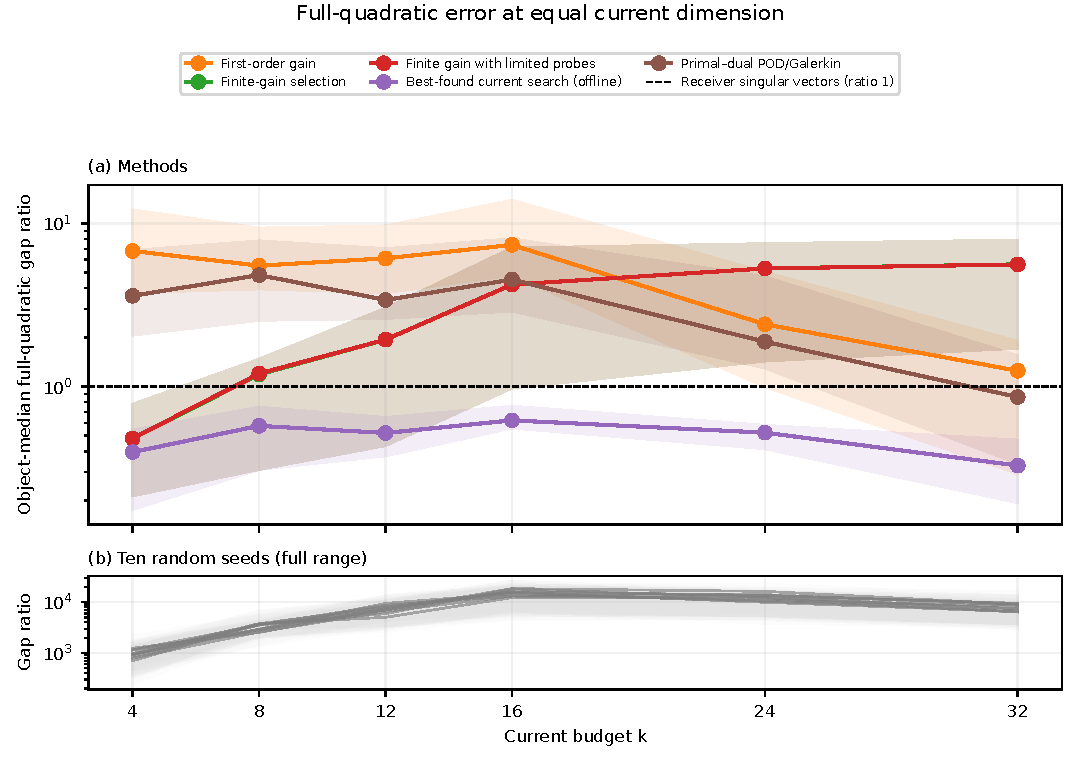
\includegraphics[width=.94\textwidth]{figures/current_design/01_fullgap_ratios.pdf}
\caption{Full-quadratic step error at equal actual current dimension. The upper panel shows object-median ratios and frozen 95\% intervals; the lower panel retains all ten random seeds over their complete range. The two finite-gain curves mostly overlap and are evaluated separately. They help at $k=4$ but lose their relative advantage as the tested budget increases. Offline current search remains below the receiver reference. These are 43 noiseless observed states from 15 objects, with missing states retained in coverage. FP64-equivalent implementation versions are combined for accuracy, while their costs remain separated.}
\label{fig:current-design}
\end{figure*}

The predeclared phase summaries also expose useful local regimes. The no-probe ratio is 1.2761 at initialization, 0.2793 before the fourth update, and 0.3597 at the last saved state. The asymmetric family ratio is 0.2793, whereas Gaussian-lobe and shell-family ratios are 1.3481 and 1.5843. These slices describe where the tested rule helps; they do not replace the failed aggregate criteria. Restricting the sensitivity analysis to the 13 complete objects leaves the finite/receiver median unchanged.

Against the particular primal--dual POD adaptation, the finite rules have aggregate ratio 0.2904 (95\% interval $[0.0785,0.5649]$). The finite/first-order policy ratio is 0.1171, but the policies also differ in their displacement and terminal swap procedure. This ratio therefore does not isolate the quadratic penalty. The controlled displacement-by-evaluation comparison below addresses those factors at the same checkpoint. The receiver control is stronger overall, and the primal--dual comparison reverses at larger budgets. No new selector reconstruction was launched because the aggregate frozen-state criteria and planned coverage were not satisfied. The supplement reports every tested control, absolute gaps, reference floors, missing cells, and version-specific marginal fees.
